
%----------------------------------------------------------------------------------------
%	PACKAGES AND OTHER DOCUMENT CONFIGURATIONS
%----------------------------------------------------------------------------------------

\documentclass{article}

\usepackage{fancyhdr} % Required for custom headers
\usepackage{lastpage} % Required to determine the last page for the footer
\usepackage{extramarks} % Required for headers and footers
\usepackage{graphicx} % Required to insert images
\usepackage{lipsum} % Used for inserting dummy 'Lorem ipsum' text into the template
\usepackage{ulem} % Required for Cross out text
\usepackage{amsmath} % Required for Math Stuff
\usepackage{enumerate}
\usepackage{amssymb}
\usepackage{hyperref,color,fullpage}

% Margins
\topmargin=-0.45in
\evensidemargin=0in
\oddsidemargin=0in
\textwidth=6.5in
\textheight=9.0in
\headsep=0.25in

\linespread{1.1} % Line spacing

% Set up the header and footer
\pagestyle{fancy}
\lhead{\hmwkAuthorName} % Top left header
\rhead{}%\firstxmark} % Top right header
%\lfoot{\lastxmark} % Bottom left footer
\cfoot{} % Bottom center footer
\rfoot{Page\ \thepage\ of\ \pageref{LastPage}} % Bottom right footer
\renewcommand\headrulewidth{0.4pt} % Size of the header rule
\renewcommand\footrulewidth{0.4pt} % Size of the footer rule

\setlength\parindent{0pt} % Removes all indentation from paragraphs

%----------------------------------------------------------------------------------------
%	DOCUMENT STRUCTURE COMMANDS
%	Skip this unless you know what you're doing
%----------------------------------------------------------------------------------------

%% Header and footer for when a page split occurs within a problem environment
%\newcommand{\enterProblemHeader}[1]{
%\nobreak\extramarks{#1}{#1 continued on next page\ldots}\nobreak
%\nobreak\extramarks{#1 (continued)}{#1 continued on next page\ldots}\nobreak
%}
%
%% Header and footer for when a page split occurs between problem environments
%\newcommand{\exitProblemHeader}[1]{
%\nobreak\extramarks{#1 (continued)}{#1 continued on next page\ldots}\nobreak
%\nobreak\extramarks{#1}{}\nobreak
%}

\setcounter{secnumdepth}{0} % Removes default section numbers
\newcounter{homeworkProblemCounter} % Creates a counter to keep track of the number of problems

\newcommand{\homeworkProblemName}{}
\newenvironment{homeworkProblem}[1][Problem \arabic{homeworkProblemCounter}]{ % Makes a new environment called homeworkProblem which takes 1 argument (custom name) but the default is "Problem #"
\stepcounter{homeworkProblemCounter} % Increase counter for number of problems
\renewcommand{\homeworkProblemName}{#1} % Assign \homeworkProblemName the name of the problem
\section{\homeworkProblemName} % Make a section in the document with the custom problem count
%\enterProblemHeader{\homeworkProblemName} % Header and footer within the environment
}{
%\exitProblemHeader{\homeworkProblemName} % Header and footer after the environment
}

\newcommand{\problemAnswer}[1]{ % Defines the problem answer command with the content as the only argument
\noindent\framebox[\columnwidth][c]{\begin{minipage}{0.98\columnwidth}#1\end{minipage}} % Makes the box around the problem answer and puts the content inside
}

\newcommand{\homeworkSectionName}{}
\newenvironment{homeworkSection}[1]{ % New environment for sections within homework problems, takes 1 argument - the name of the section
\renewcommand{\homeworkSectionName}{#1} % Assign \homeworkSectionName to the name of the section from the environment argument
\subsection{\homeworkSectionName} % Make a subsection with the custom name of the subsection
%\enterProblemHeader{\homeworkProblemName\ [\homeworkSectionName]} % Header and footer within the environment
}{
%\enterProblemHeader{\homeworkProblemName} % Header and footer after the environment
}

%----------------------------------------------------------------------------------------
%	NAME AND CLASS SECTION
%----------------------------------------------------------------------------------------

\newcommand{\hmwkTitle}{Assignment 1} % Assignment title
\newcommand{\hmwkDueDate}{Feburary 18, 2014} % Due date
\newcommand{\hmwkClass}{10-701 Machine Learning} % Course/class
\newcommand{\hmwkDueTime}{12 noon}
\newcommand{\hmwkClassInstructor}{Barnabas Poczos, Aarti Singh} % Teacher/lecturer
\newcommand{\hmwkAuthorName}{} % Your name

%----------------------------------------------------------------------------------------
%	TITLE PAGE
%----------------------------------------------------------------------------------------


\title{
\textmd{\textbf{\hmwkClass:\ \hmwkTitle}}\\
\large\vspace{0in}\Large{Due\ on\ \hmwkDueDate \ at \hmwkDueTime}\\
\vspace{0in}\large{\textit{\hmwkClassInstructor\ }}
\vspace{0.2in}
\\
\textbf{Instructions}: Failure to follow these directions may result in loss of points.
\begin{itemize}
\item{} Your solutions for this assignment need to be in a pdf format and should be submitted to the blackboard and a webpage (to be specified later) for peer-reviewing.
\item{} For the programming question, your code should be well-documented, so a TA can understand what is happening.
\item{} DO NOT include any identification (your name, andrew id, or email) in both the content and
filename of your submission.
\end{itemize}
}
\date{}

%----------------------------------------------------------------------------------------

\begin{document}

\maketitle
\vspace{-0.7in}

%----------------------------------------------------------------------------------------
%	PROBLEM 1
%----------------------------------------------------------------------------------------

\begin{homeworkProblem}[MLE, MAP, Concentration (Pengtao)] % Custom section title

\begin{homeworkSection}{1. MLE of Uniform Distributions [5 pts]} % Section within problem

Given a set of i.i.d samples $X_1, ..., X_n$ ~ $Uniform(0, \theta)$, find the maximum likelihood estimator of $\theta$.
\begin{enumerate}[(a)]
\item  Write down the likelihood function (3 pts)
\item  Find the maximum likelihood estimator (2 pts)
\end{enumerate}

\problemAnswer{ % Fill in your answer here
\lipsum[2]
}

\end{homeworkSection}
%--------------------------------------------

\vspace{-0.1in}
\begin{homeworkSection}{2. Concentration [5 pts]}
The instructors would like to know what percentage of the students like the Introduction to Machine Learning course. Let this unknown---but hopefully very close to 1---quantity be denoted by $\mu$. To estimate $\mu$, the instructors created an anonymous survey which contains this question:\\ 

"Do you like the Intro to ML course? Yes or No" \\

Each student can only answer this question once, and we assume that the distribution of the answers is i.i.d.

\begin{enumerate}[(a)]
\item  What is the MLE estimation of $\mu$? (1 pts)
\item  Let the above estimator be denoted by $\hat\mu$. How many students should the instructors ask if they want the estimated value $\hat \mu$ to be so close to the unknown $\mu$ such that 
$$
\mathbb{P}(|\hat \mu -\mu|>0.1)<0.05, \qquad(4 \textrm{pts})
$$

\end{enumerate}

\problemAnswer{ % Fill in your answer here
\lipsum[2]
}
\end{homeworkSection}



\begin{homeworkSection}{3. MAP of Multinational Distribution [10 pts]} 
You have just got a loaded 6-sided dice from your statistician friend. Unfortunately, he does not remember its exact probability distribution $p_1,p_2,...,p_6$. He remembers, however, that he generated the vector $(p_1,p_2,\ldots,p_6)$ from the following Dirichlet distribution.

$$
\mathbb{P}(p_1,p_2,\ldots,p_6)=\frac{\Gamma(\sum_{i=1}^6 u_i)}{\prod_{i=1}^6 \Gamma(u_i)} \prod_{i=1}^6 p_i^{u_i-1}\delta(\sum_{i=1}^6-1),
$$
where he chose $u_i=i$ for all $i=1,\ldots, 6$. Here $\Gamma$ denotes the gamma function, and $\delta$ is the Dirac delta.
To estimate the probabilities $p_1,p_2,\ldots,p_6$, you roll the dice 1000 times and then observe that side $i$ occurred $n_i$ times ($\sum_{i=1}^6 n_i=1000$).

\begin{enumerate}[(a)]
\item Prove that the Dirichlet distribution is conjugate prior for the multinomial distribution.
\item What is the posterior distribution of the side probabilities, $\mathbb{P}(p_1,p_2,\ldots,p_6|n_1,n_2,\ldots,n_6)$? 
\end{enumerate}

\problemAnswer{ % Fill in your answer here
\lipsum[2]
}

\end{homeworkSection}



  
%--------------------------------------------

\end{homeworkProblem}
\vspace{0.1in}
%\newpage
%----------------------------------------------------------------------------------------
%	PROBLEM 2
%----------------------------------------------------------------------------------------


\begin{homeworkProblem}[Linear Regression (Dani)] % Roman numerals

\begin{homeworkSection}{1. Optimal MSE rule [10 pts]}
Suppose we knew the joint distribution $P_{XY}$. The optimal rule
$f^*: X\rightarrow Y$ which minimizes the MSE (Mean Square Error) is given as:
$$
f^* = \arg\min_{f} \mathbb{E}[(f(X)-Y)^2]
$$
Show that $f^*(X) = \mathbb{E}[Y|X]$.

\problemAnswer{ % Fill in your answer here
\lipsum[2]
}
\end{homeworkSection}

\begin{homeworkSection}{2. Ridge Regression [10 pts]}
In class, we discussed $\ell_2$ penalized linear regression:
$$
\widehat \beta = \arg\min_{\beta} \sum^n_{i=1} (Y_i - X_i \beta)^2 + \lambda \|\beta\|^2_2
$$
where $X_i = [X_i^{(1)} \dots X_i^{(p)}]$.
\begin{itemize}
\item[]{a)}
Show that a closed form expression for the ridge estimator is $\widehat \beta = (\pmb{A}^\top \pmb{A} +\lambda \pmb{I})^{-1}\pmb{A}^\top\pmb{Y}$ where $\pmb{A} = [X_1; \dots; X_n]$
and $\pmb{Y} = [Y_1; ...; Y_n]$.
\item[]{b)}
An advantage of ridge regression is that a unique solution always exists since $(\pmb{A}^\top \pmb{A} +\lambda \pmb{I})$ is invertible. To be invertible, a matrix needs to be full rank. Argue that $(\pmb{A}^\top \pmb{A} +\lambda \pmb{I})$ is full rank by characterizing its $p$ eigenvalues in terms of the singular values of $\pmb{A}$ and $\lambda$.
\end{itemize}

\problemAnswer{ % Fill in your answer here
\lipsum[2]
}
\end{homeworkSection}

%--------------------------------------------

\end{homeworkProblem}
\vspace{0.1in}

%\newpage

%----------------------------------------------------------------------------------------
%	PROBLEM 3
%----------------------------------------------------------------------------------------

\begin{homeworkProblem}[Logistic Regression (Prashant)] % Roman numerals
\begin{homeworkSection}{1. Overfitting and Regularized Logistic Regression [10 pts]}
\begin{itemize}
\item[]{a)} Plot the sigmoid function $1/(1+e^{-wX})$ vs. $X\in \mathbb{R}$ for increasing weight $w \in \{1, 5, 100\}$. A qualitative sketch is enough. Use these plots to argue why a solution with
large weights can cause logistic regression to overfit.
\item[]{b)}
To prevent overfitting, we want the weights to be small. To achieve this,
instead of maximum conditional likelihood estimation M(C)LE for logistic regression:
$$\max_{w_0,\dots, w_d}\prod^n_{i=1} P(Y_i|X_i, w_0,\dots, w_d),$$
we can consider maximum conditional a posterior M(C)AP estimation:
$$\max_{w_0,\dots, w_d}
\prod^n_{i=1} P(Y_i|X_i, w_0,\dots, w_d) P(w_0, \dots, w_d)
$$
where $P(w_0, \dots, w_d)$ is a prior on the weights.

Assuming a standard Gaussian prior ${\cal N}(0,\pmb{I})$ for the weight vector,
derive the gradient ascent update rules for the weights.
\end{itemize}

\problemAnswer{ % Fill in your answer here
\lipsum[2]
}
\end{homeworkSection}

\begin{homeworkSection}{2. Multi-class Logistic Regression [10 pts]}
One way to extend logistic regression to multi-class (say K class labels) setting is to consider
(K-1) sets of weight vectors and define
$$
P(Y=y_k|X) \propto \exp(w_{k0}+ \sum^d_{i=1}w_{ki}X_i) \ \mbox{for} \  k = 1, \dots, K-1
$$
\begin{itemize}
\item[]{a)} What model does this imply for $P(Y=y_K|X)$?
\item[]{b)} What would be the classification rule in this case?
\item[]{c)} Draw a set of training data with three labels and the decision boundary resulting from a multi-class logistic regression. (The boundary does not need to be quantitatively correct but should qualitatively depict how a typical boundary from multi-class logistic regression would look like.)
\end{itemize}
\problemAnswer{ % Fill in your answer here
\lipsum[2]
}
\end{homeworkSection}

\end{homeworkProblem}
%\newpage
\vspace{0.1in}
%----------------------------------------------------------------------------------------
%	PROBLEM 4
%----------------------------------------------------------------------------------------

\begin{homeworkProblem}[Naive Bayes Classifier (Pulkit)] % Roman numerals
\begin{homeworkSection}{1. Naive Bayes Classification Implementation [25 pts]}
In this question, you will write a Naive Bayes classifier and verify its performance on a news-group data-set. As you learned in class, Naive Bayes is a simple classification algorithm that makes an assumption about conditional independence of features, but it works quite well in practice. You will implement the Naive Bayes algorithm (Multinomial Model) to classify a news corpus into 20 different categories. \\ \\
You have been provided with the following data files:
\begin{itemize}
\item train.data - Contains bag-of-words data for each training document. Each row of the file represents the number of occurrences of a particular term in some document. The format of each row is (docId, termId, Count).
\item train.label - Contains a label for each document in the training data.
\item test.data - Contains bag-of-words data for each testing document. The format of this file is the same as that of the train.data file.
\item test.label - Contains a label for each document in the testing data.
\end{itemize}

For this assignment, you need to write code to complete the following functions:
\begin{itemize}
\item logPrior(trainLabels) - Computes the log prior of the training data-set. (5 pts)
\item logLikelihood(trainData, trainLabels) - Computes the log likelihood of the training data-set. (7 pts)
\item naiveBayesClassify(trainData, trainLabels, testData) - Classifies the data using the Naive Bayes algorithm. (13 pts)
\end{itemize}

\underline{Implementation Notes}
\begin{enumerate}
\item We compute the log probabilities to prevent numerical underflow when calculating multiplicative probabilities. You may refer to \href{http://blog.smola.org/post/987977550/log-probabilities-semirings-and-floating-point-numbers}{this} article on how to perform addition and 
multiplication in log space. 
\item You may encounter words during classification that you haven't during training. This may be for a particular class or over all. Your code should deal with that. 
\item Be memory efficient and please do not create a document-term-matrix in your code. That would require upwards of 600MB of memory.
\end{enumerate}

Due to popular demand, we are allowing the solution to be coded in 3 languages: Octave, Julia, and Python. \\ \\
Octave is an industry standard in numerical computing. Unlike MATLAB, it is an open-source language and has similar capabilities and syntax.\\ \\
Julia is a popular new open-source language developed for numerical and scientific computing was well as beginning effective for general programming purposes. This is the first time this language is being supported in a CMU course. \\ \\
Python is an extremely flexible language and is popular in industry and the data science community. Powerful python libraries would not be available to you. \\ \\

For Octave and Julia, a blank function interface has been provided for you. However, for Python, you will need to perform the I/O for the data files  and ensure the results are written to the correct output files. \\ \\
\end{homeworkSection}


\begin{homeworkSection}{Challenge Question}
This question is not graded, but it is highly recommended that you try it.
In the above question, we are using all the terms from the vocabulary to make a prediction. This would lead to a lot of noisy features. Although it seems counter-intuitive, classifiers built from a smaller vocabulary perform better because they generalize better over unseen data. Noisy features that are not well-represented often skew the perceived distribution of words, leading to classification errors. Therefore, the classification can be improved by selected a subset of extremely effective words. 
\end{homeworkSection}

\end{homeworkProblem}
\newpage
%----------------------------------------------------------------------------------------
%	PROBLEM 5
%----------------------------------------------------------------------------------------

% To have just one problem per page, simply put a \clearpage after each problem

\begin{homeworkProblem}[Support Vector Machines (Jit) ]

\begin{homeworkSection}{1. SVM Matching [15 points]}
 
 
 \end{homeworkSection}

Figure~\ref{Fig.sixSVMs} (at the end of this
  problem) plots SVM decision boundries resulting from using different
  kernels and/or different slack penalties. In
  Figure~\ref{Fig.sixSVMs}, there are two classes of training data,
  with labels $y_i \in \{-1, 1\}$, represented by circles and squares
  respectively. The SOLID circles and squares represent the Support
  Vectors. Determine which plot in Figure~\ref{Fig.sixSVMs} was
  generated by each of the following optimization problems: (Note that
  there are 6 plots, but only 5 problems, so one plot does not match
  any of the problems). Explain your reasoning for each choice. 

\begin{enumerate}
\item 
 \begin{equation*}
\min \frac{1}{2} \mathbf{w \cdot w} + C\sum_{i=1}^{n}\xi_i
 \end{equation*}
s.t. $\forall i = 1, \cdots, n$:  \\
$\xi_i \ge 0$ \\
$(\mathbf{w \cdot x_i} + b)y_i -(1-\xi_i) \ge 0$\\
and $ C =0.1$.




\item 
 \begin{equation}
\min \frac{1}{2} \mathbf{w \cdot w} + C\sum_{i=1}^{n}\xi_i
 \end{equation}
s.t. $\forall i = 1, \cdots, n$: \\
$\xi_i \ge 0$ \\
$(\mathbf{w \cdot x_i} + b)y_i -(1-\xi_i) \ge 0$ \\
and $ C =1$.




\item 
 \begin{equation}
\max\sum_{i=1}^{n}\alpha_i - \frac{1}{2} \sum_{i, j}\alpha_i\alpha_jy_iy_j\mathbf{K}(\mathbf{x_i}, \mathbf{x_j})
 \end{equation}
s.t.  $\sum_{i=1}^{n} \alpha_iy_i = 0$; \\
$\alpha_i \ge 0, \forall i = 1, \cdots, n$; \\
where $\mathbf{K}(\mathbf{u}, \mathbf{v}) = \mathbf{u} \cdot \mathbf{v} + ( \mathbf{u} \cdot \mathbf{v})^2 $.\\



\item 
 \begin{equation}
\max\sum_{i=1}^{n}\alpha_i - \frac{1}{2} \sum_{i, j}\alpha_i\alpha_jy_iy_j\mathbf{K}(\mathbf{x_i}, \mathbf{x_j})
 \end{equation}
s.t. $\sum_{i=1}^{n} \alpha_iy_i = 0$; \\
$\alpha_i \ge 0, \forall i = 1, \cdots, n$; \\
where $\mathbf{K}(\mathbf{u}, \mathbf{v}) = \exp (-\frac{\parallel \mathbf{u}- \mathbf{v}\parallel^2}{2})$.\\



\item 
 \begin{equation}
\max\sum_{i=1}^{n}\alpha_i - \frac{1}{2} \sum_{i, j}\alpha_i\alpha_jy_iy_j\mathbf{K}(\mathbf{x_i}, \mathbf{x_j})
 \end{equation}
s.t. $\sum_{i=1}^{n} \alpha_iy_i = 0$;  \\
$\alpha_i \ge 0, \forall i = 1, \cdots, n$; \\
where $\mathbf{K}(\mathbf{u}, \mathbf{v}) = \exp (-\parallel \mathbf{u}- \mathbf{v}\parallel^2)$.\\



\end{enumerate}

\begin{figure}[H]
  \begin{center}
    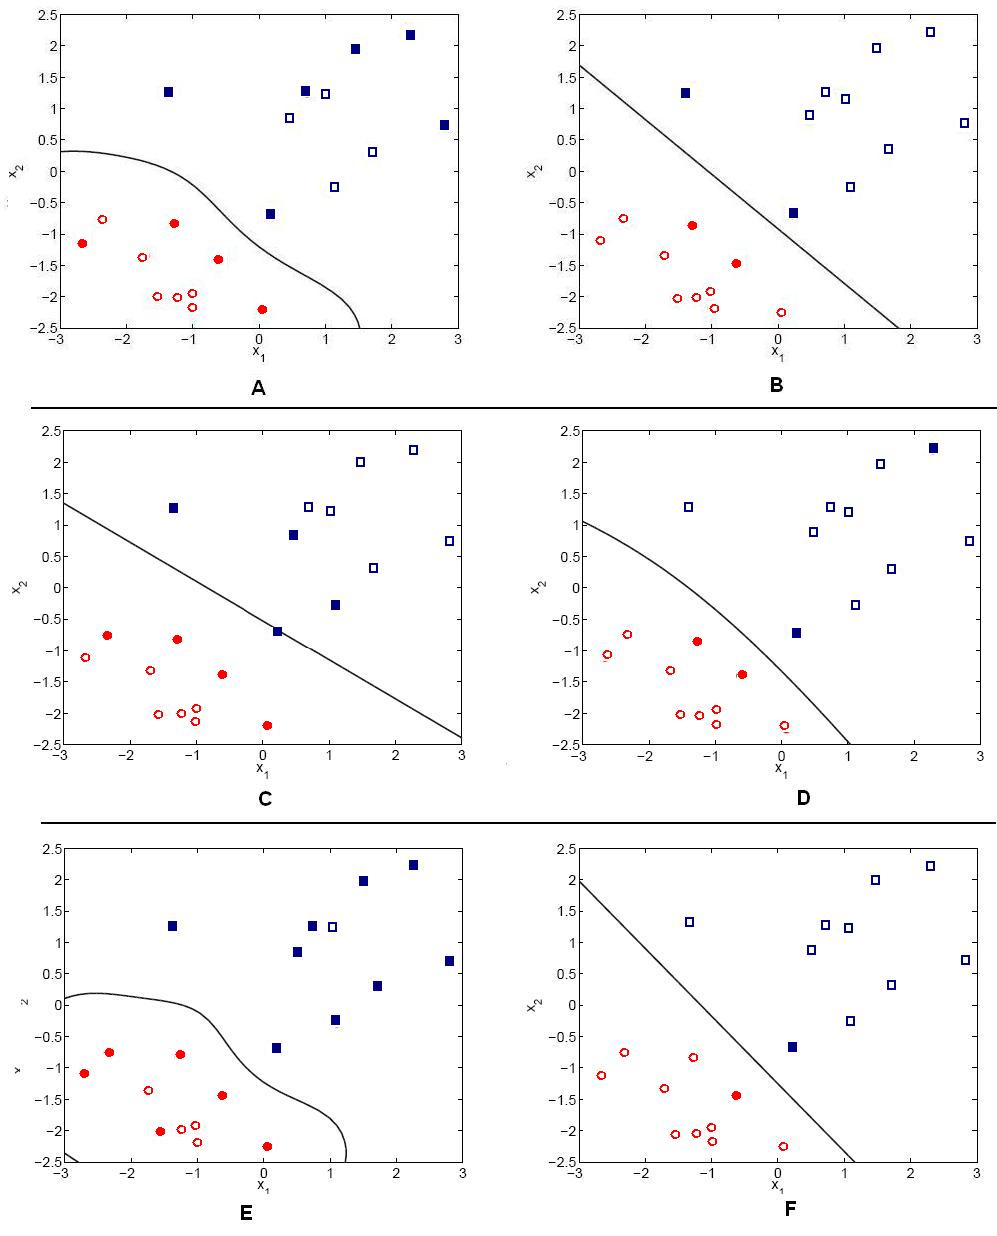
\includegraphics[width=0.98\textwidth]{./sixSVMs.jpg}
  \end{center}
  \caption{Induced Decision Boundaries}~\label{Fig.sixSVMs}
\end{figure}

 \problemAnswer{ % Fill in your answer here
\lipsum[2]
}
\end{homeworkProblem}

%----------------------------------------------------------------------------------------

\end{document}
